\section{Evaluation der Vollständigkeit}

In einem ersten Schritt wird auf die Vollständigkeit der Pellenkoft Regelmengen eingegangen. Im Folgenden wird dann die Vollständigkeit von RS-Rule genauer betrachtet.

\subsection{Vollständigkeit von RS-B0, RS-B1 und RS-B2}

Mit Hilfe des implementierten Optimierers können unterschiedliche Regelmengen ausgeführt werden. Wie in Kapitel 4 beschrieben, lassen sich neue Regeln leicht hinzufügen, Testszenarien generieren und die Ergebnisse speichern. Um die Vollständigkeit der Regelmengen zu prüfen, wurden unterschiedliche Testszenarien generiert und die einzelnen Regelmengen auf ihre Ausgabe hin überprüft. In einem ersten Schritt musste die Korrektheit der Implementierung geprüft werden.

Die Tests wurden mit Hilfe des folgenden morphologischen Kastens gebildet und ausgeführt. So konnten unterschiedliche Test Arten geprüft werden:

\begin{figure}[ht]
\centering
\resizebox{\textwidth}{!}{%
\begin{tabular}{|l|l|l|l|l|l|}
\hline
{\bf Algorithmus} & {\bf Anzahl an Knoten} & {\bf Formen} &  {\bf Initialer Baum} & {\bf Selektvität}    & {\bf Kardinalitäten} \\ \hline
RS-B0             & 5                      & Stern        & Bushy                 & Standard (0.5)       & Standard (10)        \\ \hline
RS-B1             & 7                      & Kette        & Linkstief             & Zufällig (0.0 - 1.0) & Zufällig (1 -100)    \\ \hline
RS-B2             & 10                     & Baum         & Rechtstief            &                      &                      \\ \hline
GraphRule         & 12                     & Zyklisch     &                       &                      &                      \\ \hline
\end{tabular}
}
\caption{Morthologischer Kasten zur Testgenerierung}
\label{my-label}
\end{figure}

Für jeden Test wurde das exakte Testszenario, Beobachtungen und Ergebnisse dokumentiert, um sie besser nachvollziehbar zu machen.



\newtheorem{hypo}{Hypothese} 





Einige Tests wurden ausgeführt, um die Performance und Vollständigkeit der einzelnen Regelmengen zu prüfen. Entlang der Dimensionen Regelmenge, Anzahl der Relationen, Form des Join Graphen, Form des initialen Anfragebaums, Selektivität und Kardinalität wurde ein morphologischer Kasten aufgestellt. Auf dessen Basis konnten verschiedene Tests behandelt werden. 

\subsection{Vollständigkeit der Regelmengen bei azyklischen linkstiefen Bäumen }

\begin{hypo}
Alle Regelmengen sind bei azyklischen Join-Bäumen und linkstiefen initialen-Bäumen vollständig.
\end{hypo}

\begin{figure}[ht]
  \centering
  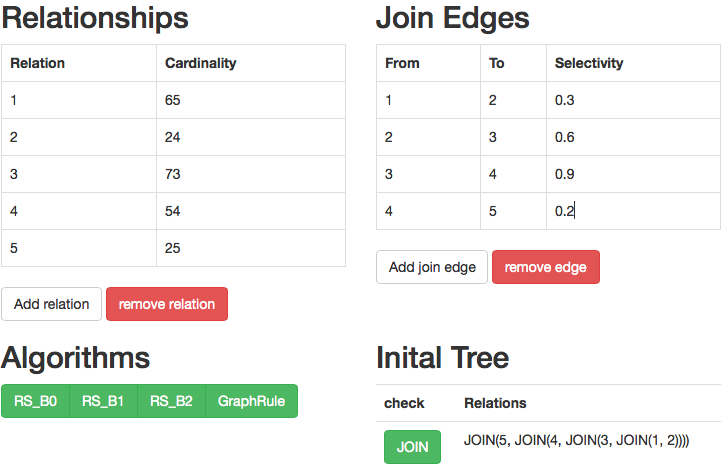
\includegraphics[width=\textwidth]{05_ResultsEvaluation/00_media/Test1.png}
  \caption{Konfiguration: Test 1}
  \label{Konfiguration:Test1}
\end{figure}

Zu diesem Zweck wurde eine Konfiguration mit fünf Relationen gewählt, die wie in Abbildung \ref{Konfiguration:Test1} zu sehen mit einander verknüpft sind.

Um festzustellen, ob alle Algorithmen für diesen speziellen Fall korrekt funktionieren, wurden zuerst alle erzeugten Pläne ausgegeben und verglichen. In einem zweiten Schritt wurden alle Äquivalenzklassen betrachtet und auf ihren Inhalt manuell geprüft.



\begin{figure}[ht]
\centering

\begin{tabular}{|l|l|l|l|}
\hline
                         & \multicolumn{3}{c|}{{\bf Result}} \\ \hline
{\bf Algorithmus}        & RS-B0     & RS-B1     & RS-B2     \\ \hline
{\bf Anzahl Bäume}       & 224       & 224       & 224       \\ \hline
{\bf Dauer}              & 28558  & 25523  & 23280  \\ \hline
\end{tabular}

\caption{Resultat: Test 1}
\label{Resultat:Test1}
\end{figure}

Wie in Tabelle \ref{Resultat:Test1} zu sehen ist, wurden je 224 unterschiedliche Bäume erzeugt. Eine Prüfung ergab, dass die Pläne, die durch die drei Regelmengen erzeugt wurden, alle gleich sind.

In einem nächsten Schritt wurden die Äuqivalenzklassen auf ihren Inhalt geprüft. In der obersten Äquivalenzklasse fanden sich die folgenden Planknoten:

\begin{itemize}
\item join(1,2345)
\item join(12,345)
\item join(123,45)
\item join(1234,5)
\item join(2345,1)
\item join(345,12)
\item join(45,123)
\item join(5,1234)
\end{itemize}

Bei diesen Planknoten handelt es sich um alle möglichen Permutationen der Äquivalenzklasse, die die Relationen 1 bis 5 repräsentiert. Auch alle anderen 34 Äquivalenzklassen wurden manuell geprüft. Das Ergebnis ist klar: Alle Permutationen wurden generiert und somit alle Pläne gefunden.

Es lässt sich also feststellen, dass alle Regelmengen in Bezug auf linkstiefe, azyklische Query Graphen mit 5 Relationen vollständig sind.

\subsection{Prüfung von azyklischen, sternförmigen Anfragen}

In einem zweiten Schritt wurde die Aussage von \cite{shanbhag2014optimizing} als Grundlage genommen, der behauptete, dass sternförmige Join-Trees zu umvollständigen Resultaten führen würden.


\begin{hypo}
Auf Basis eines azyklischen, sternförmigen Join-Trees lässt sich mit RS-B2 der Suchraum nicht vollständig erforschen.
\end{hypo}


\begin{figure}[ht]
  \centering
  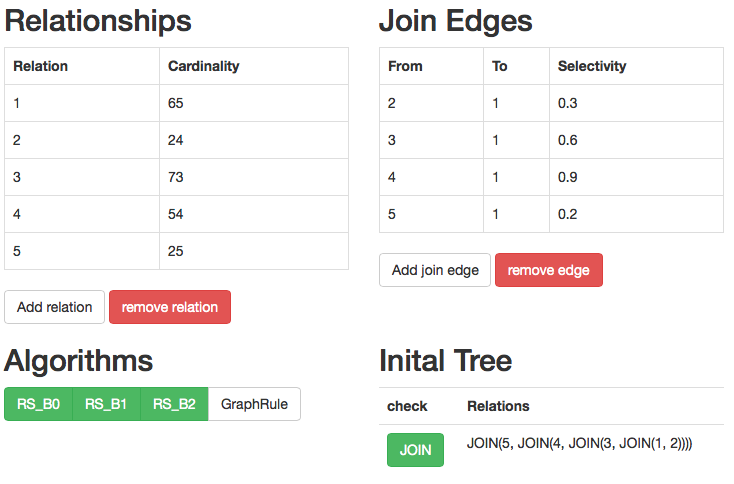
\includegraphics[width=\textwidth]{05_ResultsEvaluation/00_media/Test2.png}
  \caption{Konfiguration: Test 2}
  \label{Konfiguration:Test2}
\end{figure}


Um die Hypothese zu untersuchen, wurde eine Konfiguration gewählt, die der aus Test 1 gleicht. Einziger Unterschied sind andere Join Kanten. Wie in  Abb. \ref{Konfiguration:Test2} zu sehen, sind hier alle Knoten per Join mit Knoten 1 verbunden. Eine Sternform ergibt sich.

Nach den vorhergehenden Tests von \cite{shanbhag2014optimizing} wurde erwartet, dass durch RS-B2 nicht alle Pläne gefunden werden würden. Wie in Tabelle \ref{Result:Test2} zu sehen ist, wurden jedoch genau gleich viele Pläne mit Hilfe RS-B2 wie mit RS-B1 gefunden. 

\begin{figure}[ht]
\centering

\begin{tabular}{|l|l|l|l|}
\hline
                         & \multicolumn{3}{c|}{{\bf Result}} \\ \hline
{\bf Algorithmus}        & RS-B0     & RS-B1     & RS-B2     \\ \hline
{\bf Anzahl Bäume}       & 384       & 384       & 384       \\ \hline
{\bf Dauer}              & 66643  & 65110  & 58225   \\ \hline
\end{tabular}

\caption{Resultat: Test 2}
\label{Result:Test2}
\end{figure}


Auch die Pläne aus Test 2 wurden verglichen. Pro Regelmenge wurden die gleichen Pläne generiert. Alle 43 Äquivalenzklassen wurden geprüft und ihre Vollständigkeit festgestellt.

\begin{figure}[ht]
  \centering
  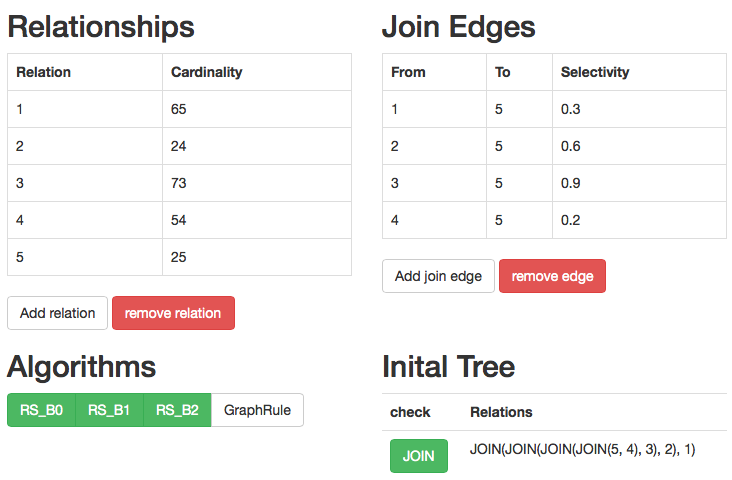
\includegraphics[width=\textwidth]{05_ResultsEvaluation/00_media/Test3.png}
  \caption{Konfiguration: Test 3}
  \label{Konfiguration:Test3}
\end{figure}


Um sicherzustellen, dass die Aussage von \cite{shanbhag2014optimizing} nicht abhängig von der Form des Baums ist, wurde ein weiterer Test durchgeführt. Dieses Mal wurde ein recht-tiefer Baum gewählt. Die Konfiguration (vgl. Abb. \ref{Konfiguration:Test3}) gleicht der vorhergehenden, ausschließlich die Join-Reihenfolge wurde verändert.

\begin{figure}[ht]
\centering
\begin{tabular}{|l|l|l|l|}
\hline
                         & \multicolumn{3}{c|}{{\bf Result}} \\ \hline
{\bf Algorithmus}        & RS-B0     & RS-B1     & RS-B2     \\ \hline
{\bf Anzahl Bäume}       & 384       & 384       & 384       \\ \hline
{\bf Dauer}              & 66643  & 65110  & 58225  \\ \hline
\end{tabular}

\caption{Resultat: Test 3}
\label{Result:Test3}
\end{figure}


Wie schon im vorhergehenden Test wurden alle Pläne geprüft. Es wurden gleich viele und die gleichen Pläne wie im vorhergehenden Fall ausgegeben. Daher kann davon ausgegangen werden, dass bei einer Menge von 5 Relationen für die Vollständigkeit nicht entscheidend ist, ob es sich initial um einen linkstiefen oder einen rechtstiefen Baum gehandelt hat.



\subsection{RS-B2 ist vollständig bei zyklischen Graphen}
Um dennoch Unvollständigkeit zu finden, wurde eine neue Hypothese aufgestellt:

Hypothese 3: RS-B2 ist bei zyklischen Join Graphen unvollständig.

Um diese Hypothese zu prüfen, wurde Test 3 herangezogen und eine neue Join-Kante zwischen 3 und 4 eingezogen (vgl. Abb. \ref{Konfiguration:Test3}. Durch diese zusätzliche Kante ist ein zyklischer Join-Graph entstanden. 


\begin{figure}[ht]
  \centering
  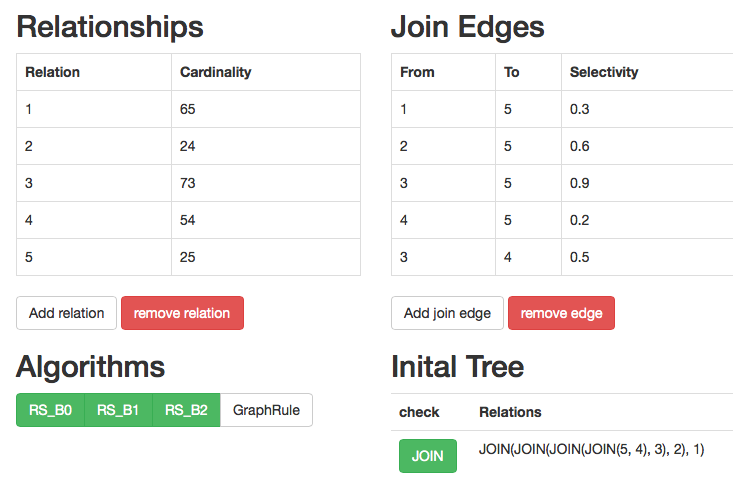
\includegraphics[width=\textwidth]{05_ResultsEvaluation/00_media/Test4.png}
  \caption{Konfiguration: Test 4}
  \label{Konfiguration:Test4}
\end{figure}

Wie erwartet, wurden weniger (ca. 50\%) Pläne gefunden (vgl. Tabelle \ref{Result:Test4}). Bei einem Vergleich fiel auf, dass gerade entlang der zyklischen-Join-Kanten weniger Pläne generiert wurden.


\begin{figure}[h]
\centering
\begin{tabular}{|l|l|l|l|}
\hline
                         & \multicolumn{3}{c|}{{\bf Result}} \\ \hline
{\bf Algorithmus}        & RS-B0     & RS-B1     & RS-B2     \\ \hline
{\bf Anzahl Bäume}       & 480       & 480       & 272       \\ \hline
{\bf Dauer}              & 60197027  & 56166774  & 28628930  \\ \hline
\end{tabular}

\caption{Resultat: Test 4}
\label{Result:Test4}
\end{figure}

Es zeigt sich mit diesem Experiment, dass RS-B2 nicht geeignet sind, um alle Pläne für einen zyklischen Join-Graphen zu erzeugen.

\subsection{RS-B2 ist Vollständig für bestimmte zyklische Join-Graphen}







\subsection{RS-B2-CPS Vollständigkeit bzgl. sternförmigen Anfragen}

Wie in Kapitel 3 gesehen wurde die Unvollständigkeit von \cite{bachelor}  mit Hilfe einer sternförmigen Anfrage nachgewiesen. Dieses Ergebnisse sollte reproduziert werden. Da diese Ergebnisse so nicht reproduzierbar waren, wird ein Erklärungsansatz vorgeschlagen.

\subsubsection{Prüfung der Ergebnisse aus Kapitel 3}
Es wurden zwei Tests durchgeführt. hierzu wurden zwei sternförmige Anfragen erzeugt. Jede Anfrage wurde ausgeführt und die Anzahl der unterschiedlichen Pläne gemessen.

\begin{figure}[h]
\centering

\begin{tabular}{|l|l|l|}
\hline
Relationen & RS-B2-CPS & RS-B1-CPS \\ \hline
5          & 284       & 284       \\ \hline
7          & 46080     & 46080     \\ \hline
\end{tabular}





\caption{Anzahl Pläne nach Regelmenge und Anzahl-Relationen}
\label{protoUnvollstaendig}
\endfigure

Im Gegensatz zu \cite{bachelor} konnte nicht festgestellt werden, dass RS-B2 schlechter als die Vergleichsregelmenge RS-B1 funktioniert.


\subsubsection{Erklärungsansatz: Pyros Expansionsalgorithmus}

Der Grund für die Abweichung mag am Expansionsalgorithmus in Pyro liegen. Der verwendete Expansionsalgorithmus (vgl. Abb. \ref{ExpandDAG}) ist vollständig für die Regelmenge RS-B1. Ob dies auch für die Regelmenge RS-B2 zutrifft, wird im folgenden an einem konkreten Beispiel geprüft.

\begin{figure}[ht]
  \centering
  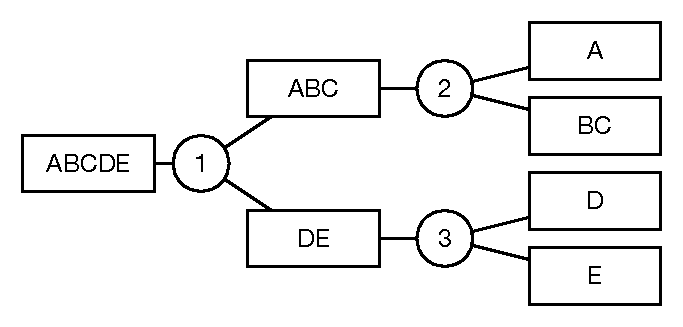
\includegraphics[scale=0.75]{05_ResultsEvaluation/00_media/PyroInital_0.pdf}
  \caption{Initialer Query Tree}
  \label{PyroInital}
\end{figure}

\begin{figure}[ht]
  \centering
  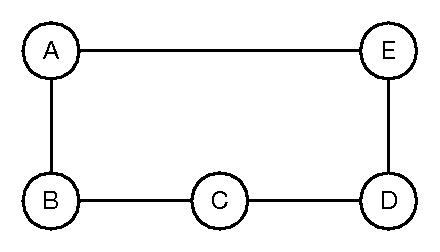
\includegraphics[scale=0.75]{05_ResultsEvaluation/00_media/PyroJoinGraph.pdf}
  \caption{Join-Graph}
  \label{PyroJoinGraph}
\end{figure}

Die Prüfung des Algorithmus erfolgt in vereinfachter Form am Beispiel des in Abb. \ref{PyroInital} dargestellten Query-Tree und Join-Graphen aus Abb. \ref{PyroJoinGraph}. Um die Darstellung zu vereinfachen, wird die Regel Kommutativität der Regelmenge nicht angewendet. Es bleiben also linke-Assoziativität, rechte-Assoziativität und Exchange erhalten.

In einem ersten Schritt sollen die Regeln auf Planknoten 1 angewendet werden. Da die untergeordneten Planknoten noch nicht expandiert wurden, muss die Expansion auf die Knoten 2 bzw. 3 angewendet werden. Da sich auf Knoten 3 keine Regel anwenden lässt, wird dieser Knoten als expandiert markiert. Auf den Knoten 2 kann Assoziativität angewendet werden. Es entsteht so der neue Knoten 4. Auf Knoten 4 lässt sich keine Regel anwenden. Alle Regeln wurden für Knoten 2 angewendet, daher kann Knoten 2 als expandiert markiert werden.

Da nun alle untergeordneten Knoten expandiert sind, kann auf Ebene von Knoten 1 alle Regeln angewendet werden. Hier ist die Anwendung von Exchange am interessantesten. Es werden die neuen Knoten 7, 8, 9, 10, 11 geschaffen. Da auf die Knoten 7, 9 keine weiteren Regeln angewendet werden dürfen, bricht der Algorithmus ab. 

\begin{figure}[ht]
  \centering
  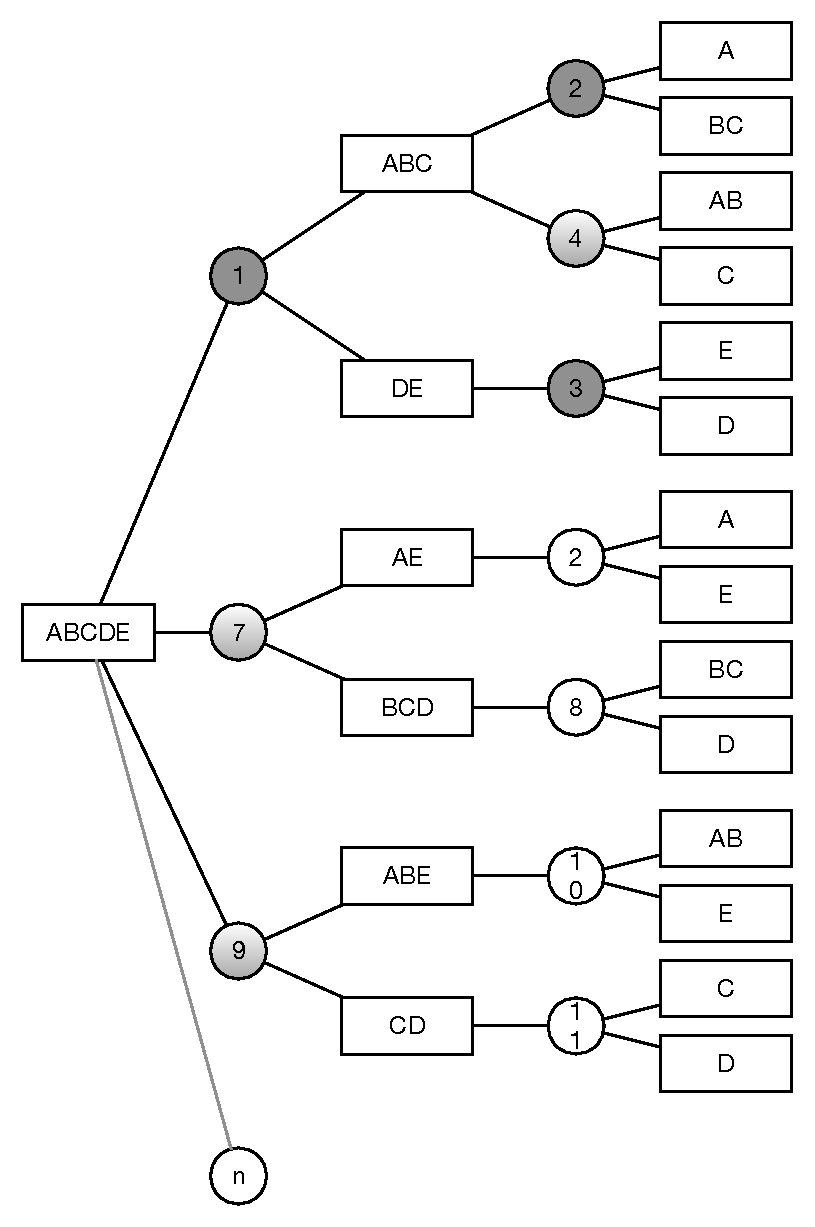
\includegraphics[scale=0.75]{05_ResultsEvaluation/00_media/PyroResult.pdf}
  \caption{Expandierter Query Tree}
  \label{ExpandedQueryTree}
\end{figure}

Wie in Abb. \ref{ExpandedQueryTree} zu erkennen, sind die Regeln nicht auf alle Teilbäume angewendet worden. Der gesamte Suchraum wurde nicht erforscht. Einer der Unterschiede zwischen dem von Pyro verwendeten und dem in Abb. \ref{Pseudocod:enumerator} gezeigten Expander ist, dass sobald ein neuer Planknoten gefunden wurde versucht wird alle Regeln, solange es möglich ist auf den gesamten Teilbaum erneut anzuwenden. So werden auch neue, untergeordnete Teilbäume in die Expansion einbezogen und der gesamte Suchraum im konkreten Beispiel erforscht.

